\subsection{Motorer og sensorer}
Test af motorer og sensorer er foretaget med både uni- og bipolære motorer som er foregået efter samme metode, hvor komponenterne er testet enkeltvis og i moduler. Der er ikke foretaget modultest af motorer for iskruning af proptrækker eller proptræk fordi åbningsmekanismen aldrig blev færdig. Der er derfor kun foretaget modultest af akserne, dog i 2 omgange, hvor unipolære motorer senere blev udskiftet med bipolære.
\\
\\
Figur \ref{fig:HW_bipolar_akse} viser test opstillingen hvor 28BYJ-48 testes på rammens akse.

\begin{figure}[H]
	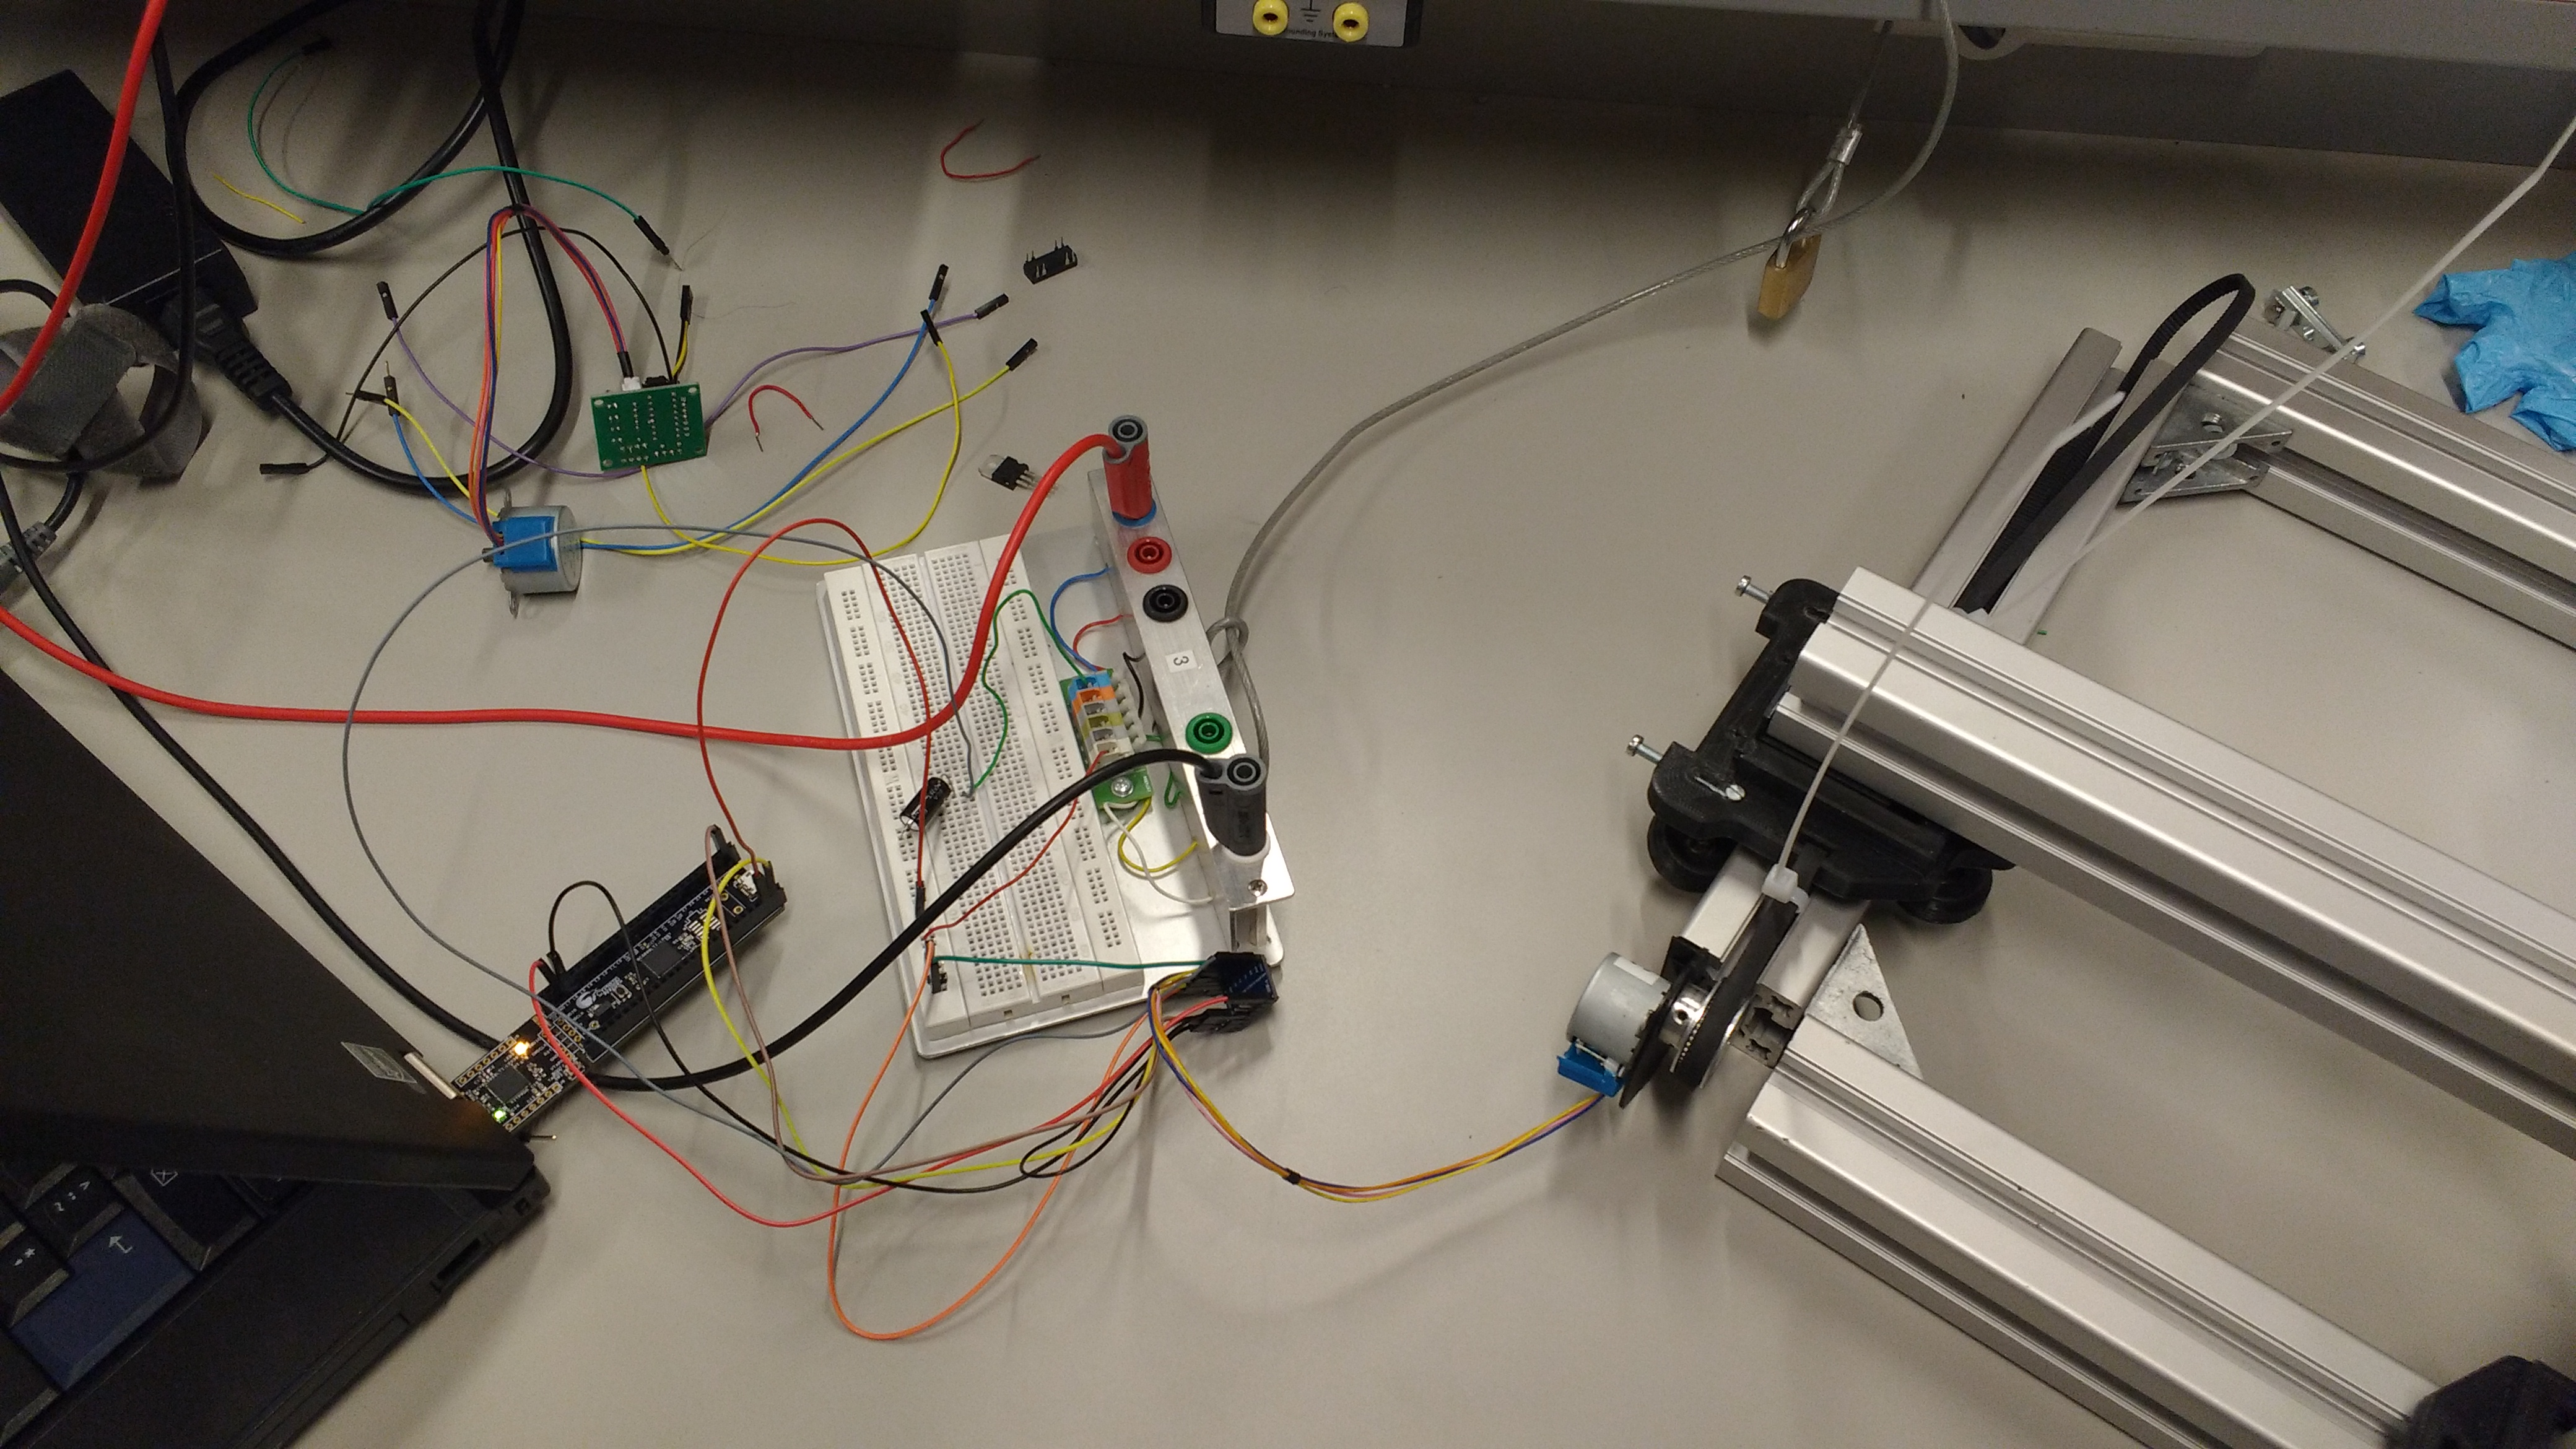
\includegraphics[scale=0.09]{tex/Test/Motor-sensor/Bipolar_test_opstilling.jpg}
	\caption{Test af 28BYJ-48 på rammens akse}
	\label{fig:HW_bipolar_akse}
\end{figure}

\noindent
Der er bygget et stativ til at teste forskellen i moment for uni- og bipolær som ses på figur \ref{fig:HW_stativ_test}.

\begin{figure}[H]
	\centerline{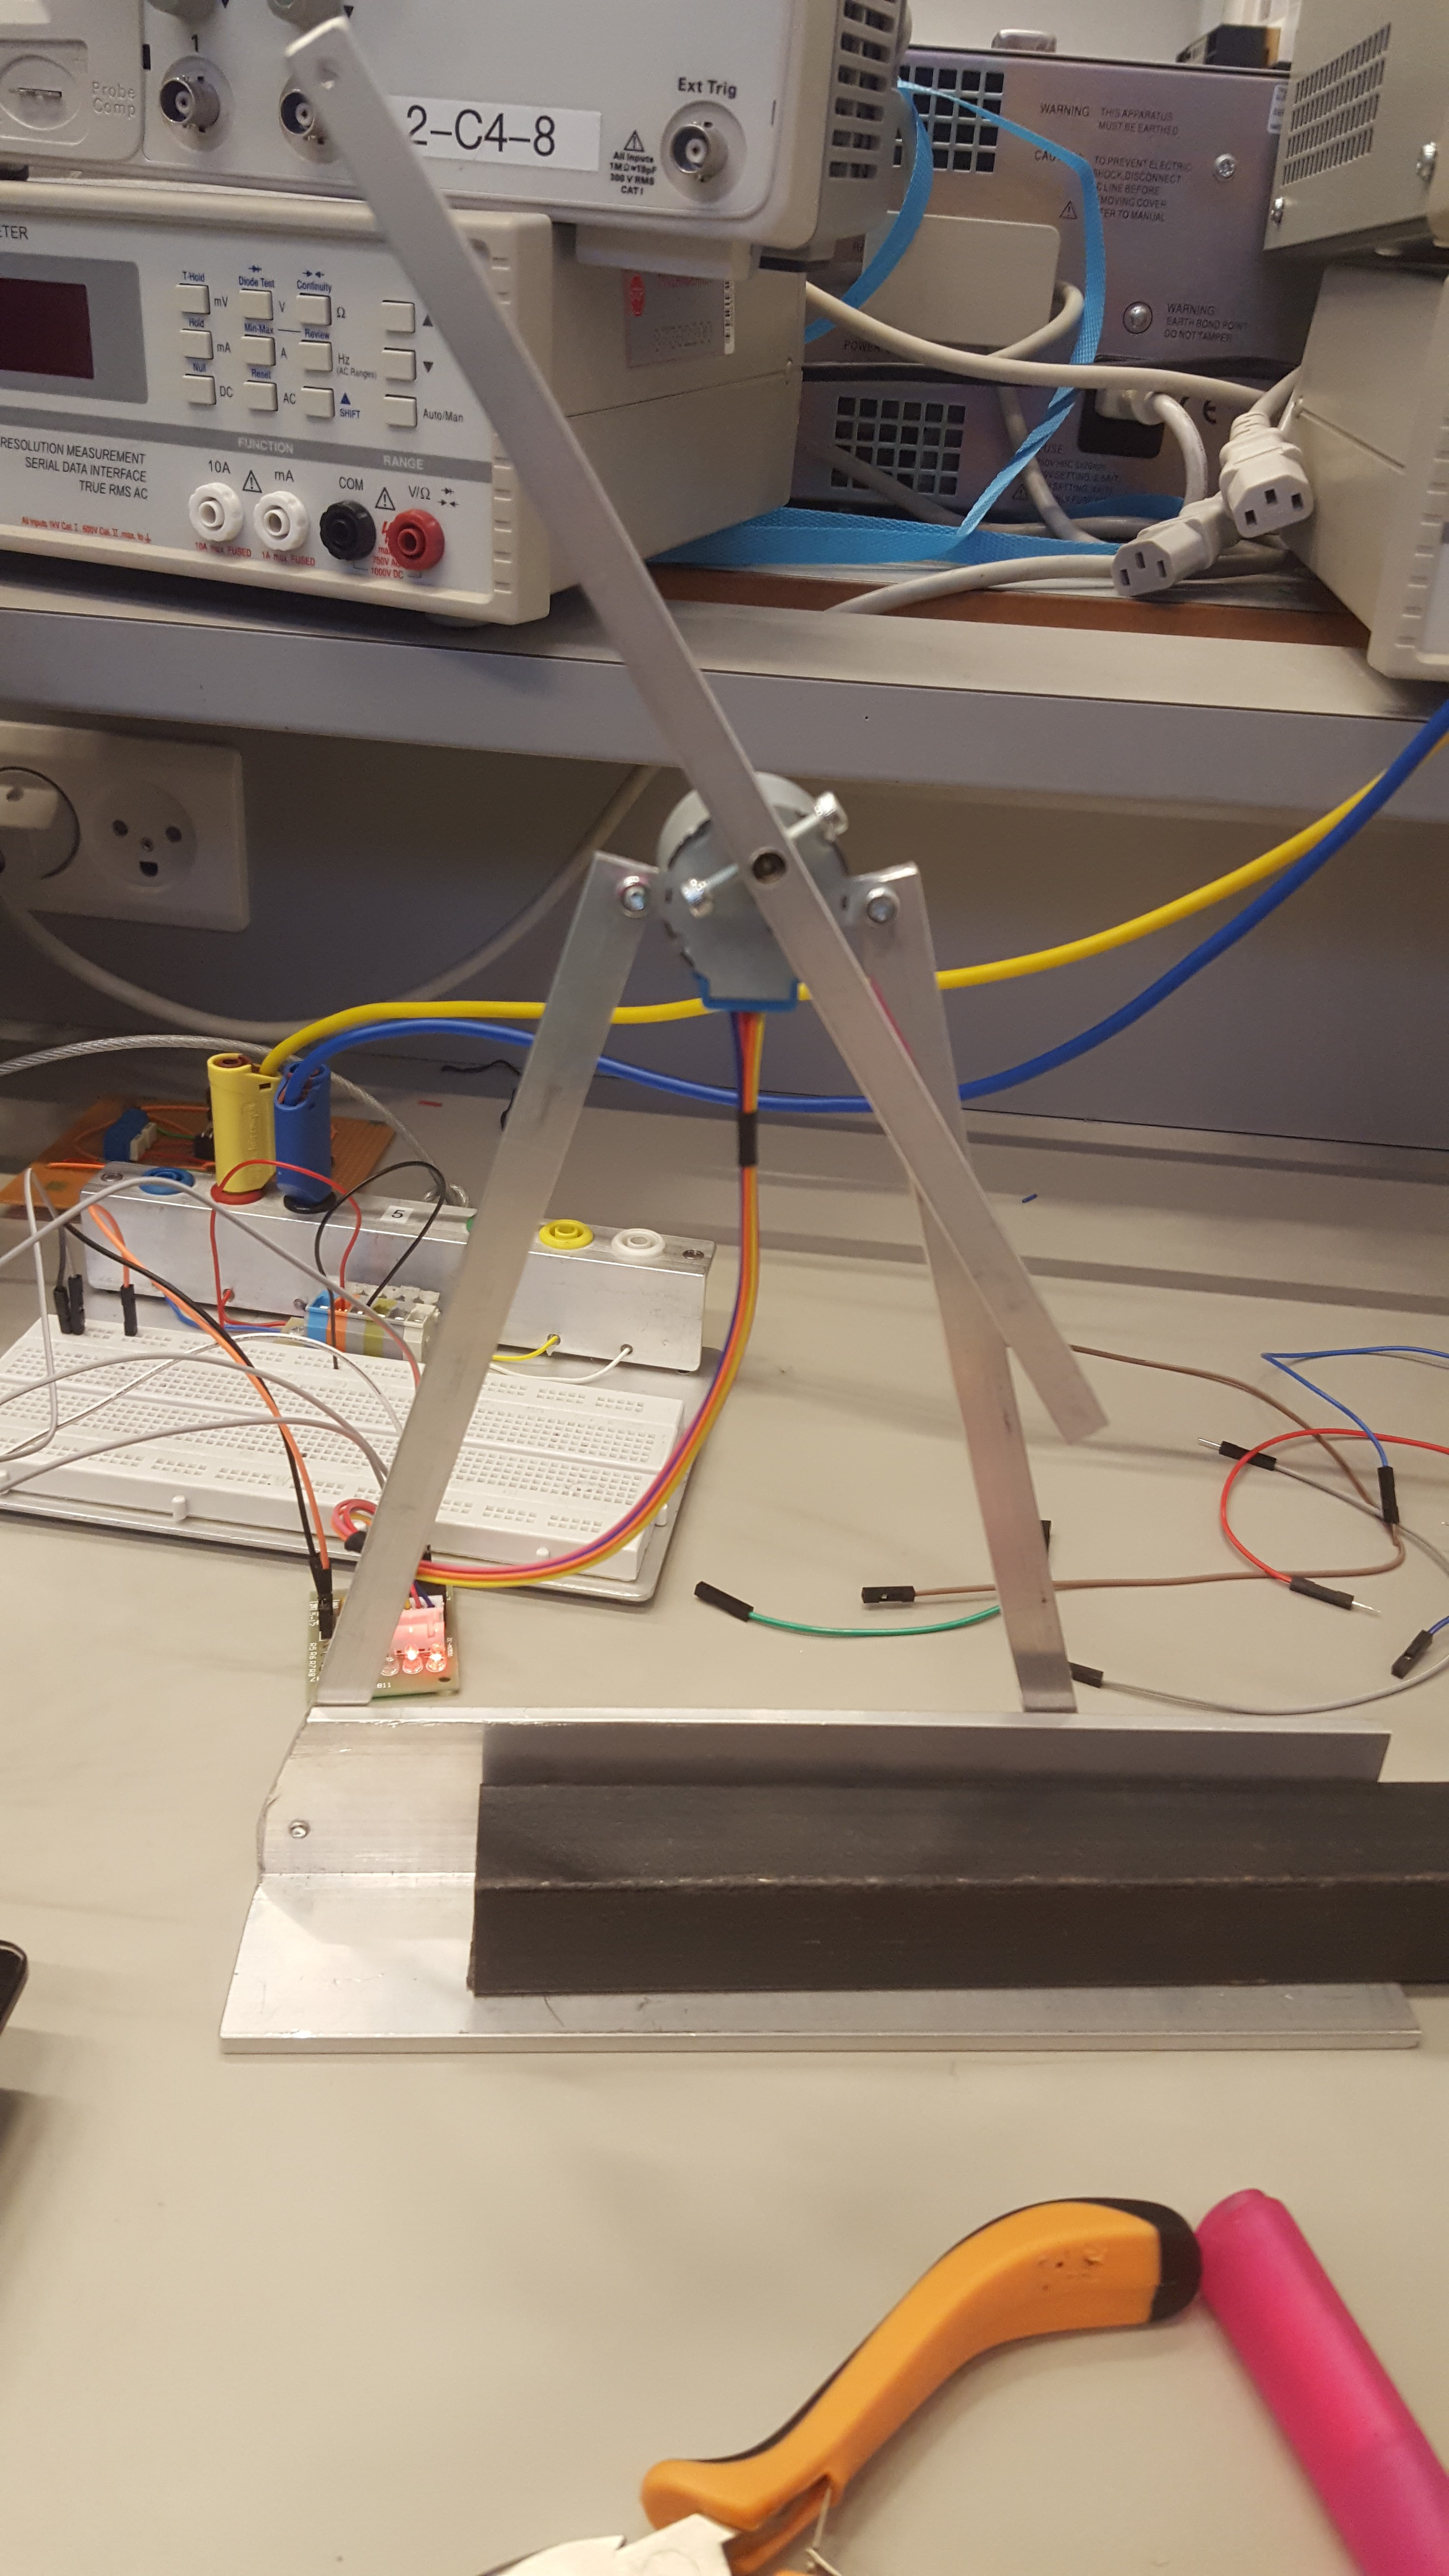
\includegraphics[scale=0.33]{tex/Test/Motor-sensor/HW_stativ_test.jpg}}
	\caption{Stativ til test af uni- og bipolær}
	\label{fig:HW_stativ_test}
\end{figure}

\noindent
Sensorerne blev testet ved at lade forskellige materialer blive detekteret på afstand af varierende størrelser.